\subsection{Pitfalls \& Fallacies}

% \begin{frame}{Threads Synchronize}
%   \begin{columns}[T] % align columns at top
%     \begin{column}{0.5\textwidth}
%     \vspace{-10pt} % Align minted to the top
%     \begin{itemize}
%         \item \emoji{no-entry} Barrier: Wait until all thread reach here
%         \begin{itemize}
%             \item Implicit barrier in parallel region
%             \item \textit{nowait} clause
%         \end{itemize}
%         \item Locking: wait until obtain the lock
%         \begin{itemize}
%             \item Often apply to data structures
%         \end{itemize}
%     \end{itemize}
%     \end{column}

%     \begin{column}{0.5\textwidth}
%     \vspace{-10pt} % Align minted to the top
%     \begin{figure}
%         \centering
%         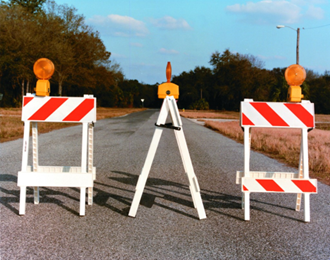
\includegraphics[width=0.5\linewidth]{day8_am/img/barrier.png}
%     \end{figure}
%     \end{column}
%   \end{columns}

% \end{frame}

\begin{frame}[fragile]{Nested Parallel Region}
    \begin{columns}[T] % align columns at top
        \begin{column}{0.3\textwidth}
            \begin{itemize}
                \item Disabled in default.
                \item Use \textit{omp\_set\_nested} to enable.
            \end{itemize}
        \end{column}

        \begin{column}{0.7\textwidth}
            \begin{minted}[fontsize=\scriptsize, highlightlines={1}]{c}
#pragma omp parallel for
for (int i = 0; i < n; i++) {
#pragma omp parallel for
    for (int j = 0; j < n; j++) {
        c[i][j] = a[i][j] + b[i][j];
    }
}
            \end{minted}
        \end{column}
    \end{columns}
\end{frame}

\begin{frame}{False Sharing}
    \begin{figure}
        \centering
        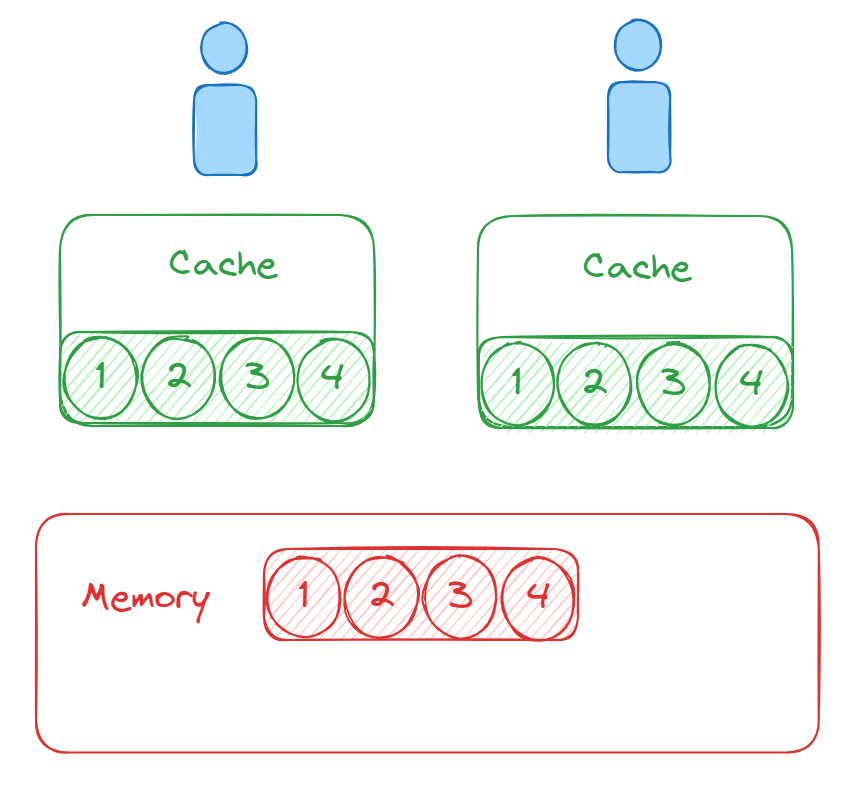
\includegraphics[width=0.5\linewidth]{day8_am/img/false_sharing.png}
    \end{figure}
\end{frame}

\begin{frame}{Takeaway: How to Optimize a program with OpenMP}
    \begin{enumerate}
        \item \textbf{Where}: Profiling
        \item \textbf{Why}: Analyze data dependency
        \item \textbf{How}: Analysis and Skills
              \begin{itemize}
                  \item Sub-task Distribution
                  \item Scheduling Strategy
                  \item Cache and Locality
                  \item Hardware Environment
              \end{itemize}
        \item Get Down to Work: Testing
    \end{enumerate}
\end{frame}

\begin{frame}{Takeaway: Tips}
    \begin{enumerate}
        \item Ensure correctness while parallelizing
        \item Be aware of overhead
        \item Check more details in official documents
    \end{enumerate}
\end{frame}